\documentclass[12pt,addpoints]{evalua}
\grado{2$^\circ$ de Secundaria}
\cicloescolar{2024-2025}
\materia{Matemáticas 2}
\unidad{3}
\title{Examen de {\color{brown}recuperación} de la Unidad}
\aprendizajes{\footnotesize%
            \item Resuelve problemas de proporcionalidad directa e inversa y de reparto proporcional.
            \item Resuelve problemas mediante la formulación y solución algebraica de ecuaciones lineales.
            \item Analiza y compara situaciones de variación lineal a partir de sus representaciones tabular, gráfica y algebraica. Interpreta y resuelve problemas que se modelan con estos tipos de variación.
            \item Verifica algebraicamente la equivalencia de expresiones de primer grado, formuladas a partir de sucesiones.      }
\author{Prof.: Julio César Melchor Pinto}
\begin{document}
\begin{questions}

      \question[4]{Contesta las siguientes preguntas:

            % \begin{multicols}{2}
            \begin{parts}
                  \part El número de goles en las últimas 3 temporadas de un delantero fueron: 22, 26 y 31, \\ \textbf{¿cuál es el promedio de goles por temporada?}
                  % \fillin[26.33][2cm]

                  \begin{solutionbox}{1.8cm}
                        Para encontrar el promedio sumamos el total de goles en esas temporadas y luego dividimos esa suma por el número de temporadas. En este caso, el promedio es
                        $(22+26+31)/3=26.33$
                  \end{solutionbox}

                  % \part En un grupo de 11 personas se registraron los siguientes pesos: 62, 64, 65, 59, 68, 72, 77, 71, 82, 69 y 76 kg. ¿Cuál es el promedio de los pesos?
                  % % \fillin[69.54][2cm]

                  % \begin{solutionbox}{2cm}
                  %       Al sumar los pesos: 62 + 64 + 65 + 59 + 68 + 72 + 77 + 71 + 82 + 69 + 76 = 765 kg, y dividir por 11 personas, obtenemos un promedio de aproximadamente 69.55 kg.
                  % \end{solutionbox}

                  part Las edades de un grupo de personas son: 44, 41, 47, 48, 44, 39, 45, 49, 44 y 47 años. \\ \textbf{¿Cuál es la mediana de las edades?}
                  % \fillin[44.5][2cm]

                  \begin{solutionbox}{1.2cm}
                        Ordenando los datos se obtiene: $\left\{39, 41, 44, 44, 44, 45, 47, 47, 48, 49 \right\} \therefore$ Mediana es 44.5
                  \end{solutionbox}
            \end{parts}
            % \end{multicols}
      }

      \question[2]{Escribe los términos faltantes de las siguientes sucesiones aritméticas:

            \begin{multicols}{2}
                  \begin{parts}
                        \part 56, 50, 44, \fillin[38][0.5cm], \fillin[32][0.5cm], \fillin[26][0.5cm], \dots
                        \part 33, 41, 49, \fillin[57][0.5cm], \fillin[65][0.5cm], \fillin[73][0.5cm], \dots
                  \end{parts}
            \end{multicols}%
      }

      \newpage

      \question[3]{Los resultados de una encuesta se muestran en la siguiente gráfica de barras:

            \begin{multicols}{2}
                  \begin{parts}
                        \part  ¿Cuántas personas participaron en la encuesta?
                        \fillin[95][2cm]
                        \part  ¿Cuál es la fruta menos preferida por las personas?
                        \fillin[Naranja][2cm]
                        \part  ¿Cuál es la fruta preferida por las personas?
                        \fillin[Manzana][2cm] \\[3em]
                  \end{parts}

                  \columnbreak%

                  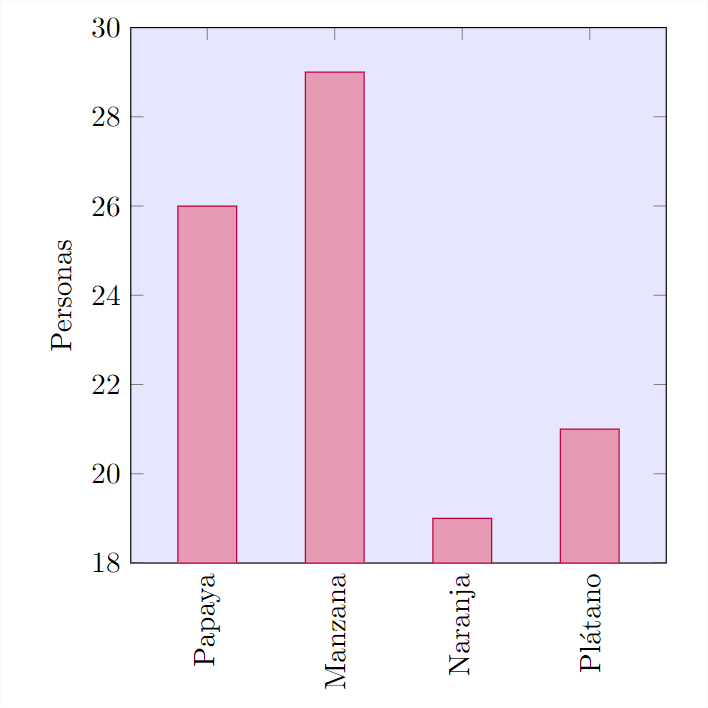
\includegraphics[width=1.1\linewidth]{mexmat00001.png}
            \end{multicols}
      }

      \question[8]{Resuelve los siguientes problemas:

            % \begin{multicols}{2}
            \begin{parts}
                  %             \part 
                  \part En una urna hay 8 pelotas moradas, 12 naranjas, 7 rojas, 11 azules y 7 blancas. \\ \textbf{Calcula la probabilidad de sacar una pelota blanca.}

                  \begin{solutionbox}{2cm}
                  \end{solutionbox}

                  \part Si 8 trabajadores construyen un muro en 15 horas, \\ \textbf{¿cuánto tardarán 5 trabajadores en construir el mismo muro?}% 

                  \begin{solutionbox}{2cm}
                        \fillin[24][0.5cm]
                  \end{solutionbox}

                  %             \part Un grifo tiene un caudal de salida de 18 litros por minuto y tarda 14 horas en llenar un tanque. ¿Cuánto tardaría si el caudal fuera de 7 litros por minuto?
                  %             \fillin[36][0.5cm]

                  %             \begin{solutionbox}{2cm}
                  %             \end{solutionbox}
            \end{parts}
            % \end{multicols}
      }

      \question[2]{Determina la diferencia de las siguientes sucesiones aritméticas:

            \begin{multicols}{2}
                  \begin{parts}
                        \part $-23,-15,-7,1,9,17,\ldots$\\[1em]
                        d=\fillin[$8$][0in]
                        \part $7,9,11,13,15,17,\ldots$\\[1em]
                        d=\fillin[$2$][0in]
                  \end{parts}
            \end{multicols}
      }


      \newpage
      \question[10]{Determina si las siguientes tablas de datos son o no son una relación proporcional. Si es una relación proporcional obten la constante de proporcionalidad:


            \begin{minipage}[t]{0.3\linewidth}
                  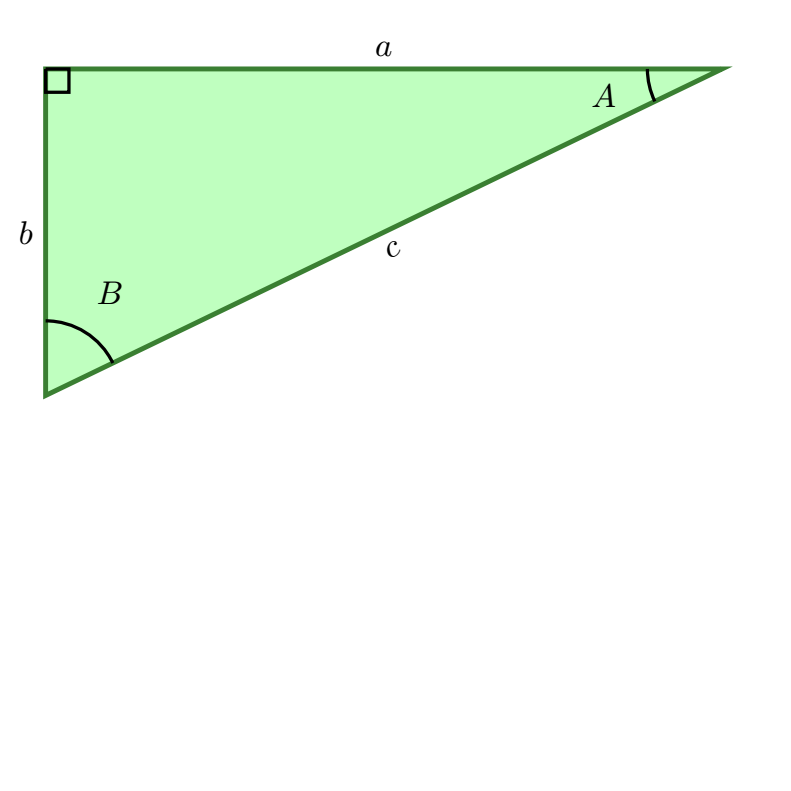
\includegraphics[width=0.9\textwidth]{mex_0072.png}
            \end{minipage}\hfill%
            \begin{minipage}[b]{0.7\linewidth}
                  \begin{oneparchoices}\Large
                        \CorrectChoice Proporcional
                        \choice No proporcional
                  \end{oneparchoices}
                  \begin{solutionbox}{3cm}
                        $43.2\div 18=2.4$\\[-0.2em]
                        $33.6\div 14=2.4$\\[-0.2em]
                        $24\div 10=2.4$\\[-0.2em]
                        $14.4\div 6=2.4$\\[-0.2em]
                        $4.8\div 2=2.4$\\[-0.2em]
                        $\therefore$ es una relación proporcional y la constante de proporcionalidad es
                  \end{solutionbox}
            \end{minipage}

            \begin{minipage}[b]{0.7\linewidth}
                  \begin{oneparchoices}\Large
                        \CorrectChoice Proporcional
                        \choice No proporcional
                  \end{oneparchoices}
                  \begin{solutionbox}{3.5cm}\small%

                        \begin{multicols}{2}
                              $\frac{16}{5}\div  4=\frac{4}{5}$\\[0.3em]
                              $\frac{32}{5}\div  8=\frac{4}{5}$\\[0.3em]
                              $\frac{48}{5}\div 12=\frac{4}{5}$\\[0.3em]
                              $\frac{64}{5}\div 16=\frac{4}{5}$\\[0.3em]
                              $16\div 20=\frac{4}{5}$

                              \columnbreak%  

                              $\therefore$ La constante de proporcionalidad es $\dfrac{4}{5}$.
                        \end{multicols}
                  \end{solutionbox}
            \end{minipage}\hfill%
            \begin{minipage}[t]{0.3\linewidth}
                  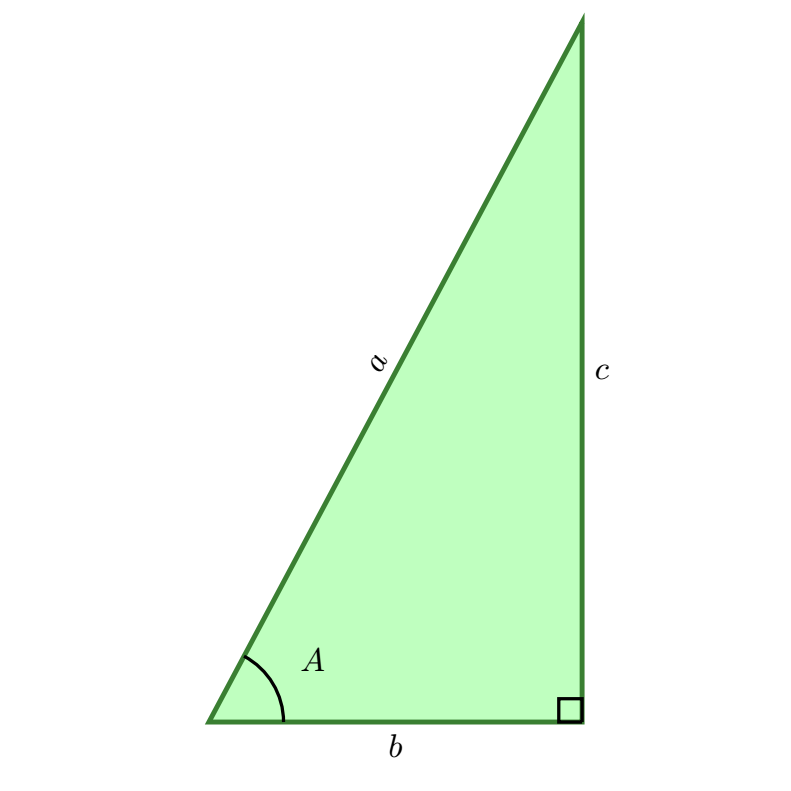
\includegraphics[width=0.9\textwidth]{mex_0073.png}
            \end{minipage}



            %       \end{parts}
            % \end{multicols}
      }

      \question[10]{Encuentra el \textit{n-ésimo} término de la siguientes sucesiones aritméticas:

            % \begin{multicols}{2}
            \begin{parts}
                  \part Calcula  el término número 44 de la siguiente sucesión aritmética: \[a_n=-3n-15\]

                  \begin{solutionbox}{2cm}
                        \[a_{44}=-3(44)-15=-132-15=-147\]
                  \end{solutionbox}

                  \part Calcula el término número 28 de la siguiente sucesión aritmética: \[-69,-72,-75,-78,-81,\ldots\]
                  \begin{solutionbox}{2cm}
                        \[-3(28)-66=-84-66=-150\]
                  \end{solutionbox}

            \end{parts}
            % \end{multicols}
      }

      \question[10]{Determina el término general de las siguientes sucesiones aritméticas:
            % \begin{multicols}{2}
            %       \begin{parts}
            %             \part $40,35,30,25,20,\ldots$ \fillin[$5-5n$][1in]
            % \part 
            \[-2,-6,-10,-14,-18,\ldots\]

            \begin{solutionbox}{1cm}
                  \fillin[$-4n+2$][0in]
            \end{solutionbox}

            % \end{parts}
            % \end{multicols}
      }





      \question[10]{Encuentra el valor numérico de la siguiente expresión:

      % \begin{multicols}{2}
      %       \begin{parts}
      %             \part $ \dfrac{m-p}{n}$ cuando $m=8$, $n=5$ y $p=-2$.

      %             \begin{solutionbox}{1.6cm}\footnotesize%
      %                   $\dfrac{m-p}{n}=\dfrac{8-(-2)}{5}=\dfrac{8+2}{5}=\dfrac{10}{5}=$ \fillin[2][0cm]
      %             \end{solutionbox}

      %             \part 
      \[a^{2}-2ab+b^{2} \qquad \text{ cuando } \qquad a=-4 \text{ y } b=-7\]

      \begin{solutionbox}{3cm}
            $a^{2}-2ab+b^{2}=(-4)^{2}-2(-4)(-7)+(-7)^{2}=16-56+49=$ \fillin[9][0cm]
      \end{solutionbox}
      %       \end{parts}
      % \end{multicols}
      }

      \question[10]{Resuelve la siguiente ecuación:

            % \begin{multicols}{3}
            %       \begin{parts}
            %             \part $ -x-2=15 $

            %             \begin{solutionbox}{3.5cm}\footnotesize%
            %                   \begin{align*}
            %                         -x-2 & = 15                \\
            %                         -x   & =15+2               \\
            %                         -x   & =17                 \\
            %                         x    & = \frac{17}{-1}=-17
            %                   \end{align*}
            %             \end{solutionbox}

            %             \part $ 11x-33=55 $

            %             \begin{solutionbox}{3.5cm}\footnotesize%
            %                   \begin{align*}
            %                         11x-33 & = 55            \\
            %                         11x    & =55+33          \\
            %                         11x    & =88             \\
            %                         x      & = \frac{88}{11}
            %                   \end{align*}
            %             \end{solutionbox}
            % \part
            \[-5x+9=-8x+3\]

            \begin{solutionbox}{3cm}\footnotesize%
                  \begin{align*}
                        -5x+9   & =-8x+3 \\
                        -5x     & =-8x-6 \\
                        -5x +8x & =-6    \\
                        3x      & =-6    \\
                        x       & =-2
                  \end{align*}
            \end{solutionbox}
            % \end{parts}
            % \end{multicols}
      }

      \question[16]{Utilizando el m\'etodo de tu preferencia, encuentra el valor de $x$ y $y$ para
            el siguiente sistema de ecuaciones lineales:

            \begin{align*}
                  \frac{3}{5}x+\frac{1}{4}y & =  2   \\[1em]
                  x-5y                      & =   25
            \end{align*}

            \begin{solutionbox}{6cm}
                  $x=5$, $y=-4$
            \end{solutionbox}
            % \vspace{4cm}
            % \end{parts}
            % \end{multicols}
      }

      \newpage

      \question[15]{Numera correctamente los pasos para resolver un sistema de dos ecuaciones con dos inc\'ognitas por los m'etodos a continuaci\'on:
            \begin{parts}
                  \part M\'etodo de sustitución:
                  \begin{checkboxes}
                        \choice \fillin[2][0cm] Sustituir la expresi\'on de esta inc\'ognita en la otra ecuaci\'on para obtener una ecuaci\'on con una sola inc\'ognita.
                        \choice \fillin[4][0cm] Sustituir el valor obtenido en la ecuaci\'on en la que aparec\'ia la inc\'ognita despejada.
                        \choice \fillin[1][0cm] Despejar una inc\'ognita en una de las ecuaciones.
                        \choice \fillin[5][0cm] Sustituir los valores en las ecuaciones originales para comprobar que son la soluci\'on.
                        \choice \fillin[3][0cm] Resolver la ecuaci\'on resultante.
                  \end{checkboxes}

                  \part M\'etodo de suma-resta:
                  \begin{checkboxes}
                        \choice \fillin[4][0cm] Sustituir el valor obtenido en una de las ecuaciones iniciales y resolverla.
                        \choice \fillin[1][0cm] Multiplicar una o ambas ecuaciones por los n\'umeros necesarios para realizar la eliminaci\'on bajo la suma o resta.
                        \choice \fillin[5][0cm] Sustituir los valores en las ecuaciones originales para comprobar que son la soluci\'on.
                        \choice \fillin[2][0cm] Sumar o restar las ecuaciones para eliminar una de las inc\'ognitas.
                        \choice \fillin[3][0cm] Resolver la ecuaci\'on resultante.
                  \end{checkboxes}


                  \part M\'etodo de igualaci\'on:
                  \begin{checkboxes}
                        \choice \fillin[5][0cm] Sustituir los valores en las ecuaciones originales para comprobar que son la soluci\'on.
                        \choice \fillin[3][0cm] Resolver la ecuaci\'on resultante.
                        \choice \fillin[2][0cm] Igualar las expresiones para obtener una ecuaci\'on con una inc\'ognita
                        \choice \fillin[1][0cm] Despejar la misma inc\'ognita en ambas ecuaciones.
                        \choice \fillin[4][0cm] Sustituir el valor obtenido en cualquiera de las dos expresiones en las que aparec\'ia despejada la otra inc\'ognita.
                  \end{checkboxes}
            \end{parts}
      }

      % \question[10]{Resuelve el siguiente sistema de ecuaciones lineales con decimales:

      %       \begin{align*}\Large%
      %             -0.2x+0.4y= & 0.6 \\
      %             x+2y=       & -3
      %       \end{align*}

      %       \begin{solutionbox}{5cm}
      %             $x=-3$, $y=0$
      %       \end{solutionbox}
      % }
\end{questions}
\end{document}